\documentclass{article}
\textheight 23.5cm \textwidth 15.8cm
%\leftskip -1cm
\topmargin -1.5cm \oddsidemargin 0.3cm \evensidemargin -0.3cm
%\documentclass[final]{siamltex}

\usepackage{verbatim}
\usepackage{fancyhdr}
\usepackage{graphicx}

%\pagestyle{fancy} \lhead{FDM Homework Template} \chead{}
%\rhead{\bfseries Yan XU}
%
%\lfoot{} \cfoot{} \rfoot{\thepage}
%\renewcommand{\headrulewidth}{0.4pt}
%\renewcommand{\footrulewidth}{0.4pt}
%

%利用TEX排版系统的CTEX中文套装
\usepackage[UTF8,noindent]{ctex}
%等式对齐
\usepackage{amsmath}
\usepackage{amssymb}

\title{Poisson Image Editing}
\author{陈柯}

\begin{document}
	\maketitle
	
	\section{目的}
	1. 实现 Siggraph 2003 论文 “Poisson Image Editing” 的算法
	
	2. 实现多边形扫描转换算法。
	
	3. 学习使用图像库 OpenCV。
	
	\section{算法原理}
	
	\subsection{Poisson solution to guided interpolation}
	\begin{figure}[htb]
		\begin{center}
			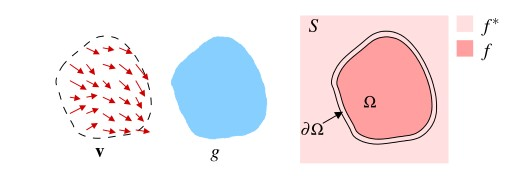
\includegraphics[width=6in]{Guided interpolation notations.jpg}
		\end{center}
	\end{figure}
	如图,$S$为$\mathbb{R}^2$中的一个闭集,是我们研究的图像的定义域。$\Omega$为$S$的
	一个闭子集,它有边界$\partial\Omega$。$f^*$是已知的定义在
	$S\backslash\Omega^{\circ}$上的标量函数,$f$是未知的定义在$\Omega^{\circ}$上的
	标量函数。$\mathbf{v}$是已知的定义在$\Omega$上的向量场。
	
	$f^*$在$\Omega$上最简单的插值$f$就是膜插值(membrane interpolant),即极小化问题:
	\begin{equation}\label{membrane}
		\min_f\iint_{\Omega}\vert\nabla f\vert^2\enspace\text{with}\enspace 
		f\vert_{\partial\Omega}=f^*\vert_{\partial\Omega}
	\end{equation}
	其解为
	\begin{equation}\label{membrane_sol}
		\Delta f=0\enspace\text{over}\enspace\Omega,\enspace\text{with}\enspace 
		f\vert_{\partial\Omega}=f^*\vert_{\partial\Omega}
	\end{equation}
	这个方法会带来模糊等问题。我们将$(\ref{membrane})$改进为
	\begin{equation}\label{extended}
		\min_f\iint_{\Omega}
		\vert\nabla f-\mathbf{v}\vert^2\enspace\text{with}\enspace 
		f\vert_{\partial\Omega}=f^*\vert_{\partial\Omega}
	\end{equation}
	其唯一解为
	\begin{equation}\label{extended_sol}
		\Delta f=\text{div}\mathbf{v}\enspace\text{over}\enspace\Omega,
		\enspace\text{with}\enspace 
		f\vert_{\partial\Omega}=f^*\vert_{\partial\Omega}
	\end{equation}

	为了实际的操作,我们将
	$(\ref{extended})$和$(\ref{extended_sol})$改为离散版本。
	$S$和$\Omega$是无限离散像素网格上定义的有限点集。对于每个$S$上的像素$p$,$N_p$为
	$p$在$S$中的上下左右4个相邻像素,符号$\langle p,q\rangle$代表$q\in N_p$。此时则
	有$\partial\Omega=\{p\in S\backslash\Omega:N_p\cap\Omega\neq\emptyset\}$。令
	$f_p$为$f$在$p$处的值。我们的任务就是去计算$f\vert_{\Omega}=\{f_p,p\in\Omega\}$
	
	将$(\ref{extended})$离散化,可得
	\begin{equation}\label{discrete}
		\min_{f\vert_{\Omega}}
		\sum_{\langle p,q\rangle\cap\Omega\neq\emptyset}
		(f_p-f_q-v_{pq})^2,\text{ with }f_p=f_p^*,\text{ for all 
		}p\in\partial\Omega
	\end{equation}
	其中$v_{pq}=\textbf{v}(\frac{p+q}{2})\cdot\overrightarrow{pq}$。其解为
	\begin{equation}\label{discrete_sol}
		\text{ for all }p\in\partial\Omega,\enspace\vert N_p\vert 
		f_p-\sum_{q\in N_p\cap\Omega}f_q=\sum_{q\in N_p\cap\partial\Omega}f_q^*
		+\sum_{q\in N_p}v_{pq}
	\end{equation}

	\subsection{Seamless cloning}
	\subsubsection{Importing gradients}
	一个基本的选择就是选取$\textbf{v}=\nabla g$,此时有$v_{pq}=g_p-g_q$。

	\subsubsection{Mixing gradients}
	上述的方法不会在$\Omega$中保留目标图像$f^*$中的任何痕迹。然而在某些情况下,我们需
	要将$f^*$和$g$的属性结合起来,例如在一个有纹理或杂乱的背景上添加有孔的物体,或部分
	透明的物体。
	
	Possion方法可以允许$\textbf{v}$为非保守梯度场,这将带来更加引人注目的效果。在
	$\Omega$的每个点处,我们保留$f^*$和$g$中变化更强烈的信息,即取
	\begin{eqnarray}
		\text{ for all }x\in\Omega,\enspace\textbf{v}(\textbf{x})=\left\{
		\begin{array}{lcl}
		\nabla f^*(\textbf{x})&	&\text{if }\vert\nabla 
		f^*(\textbf{x})\vert>\vert\nabla g(\textbf{x})\vert\\
		\nabla g(\textbf{x})&	&\text{otherwise} 
		\end{array} \right.
	\end{eqnarray}





	\subsection{多边形的扫描转换算法}
	多边形的扫描转换算法是多边形区域光栅化(求解一个平面多边形区域的内部像素)的经典算
	法,可在任何一本计算机图形学的课本上都能找到,网上也有不少详细介绍资料。
	
	算法的基本思想是:通过维持一个特别的数据结构(结构中保存扫描线与多边形的交点)进行
	填充。
	\begin{figure}[htb]
		\begin{center}
			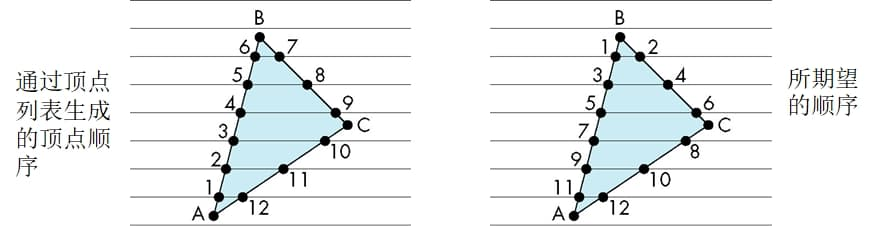
\includegraphics[width=4in]{scan_line.jpg}
		\end{center}
	\end{figure}
	
	\clearpage
	\section{实现结果}
	\subsection{UI设计}
	\begin{figure}[htb]
		\begin{center}
		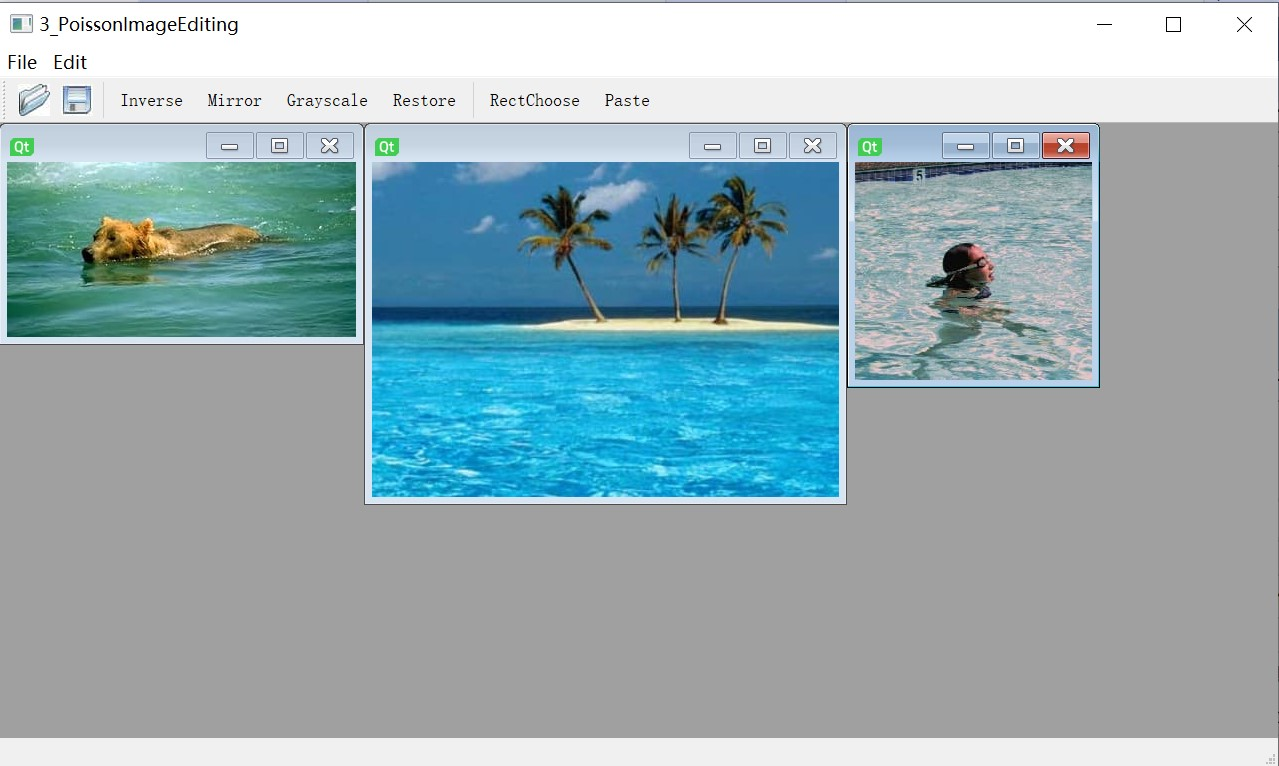
\includegraphics[width=4in]{ui.jpg}
		\end{center}
	\end{figure}


	\subsection{possion方法}
	\begin{figure}[htb]
		\begin{center}
			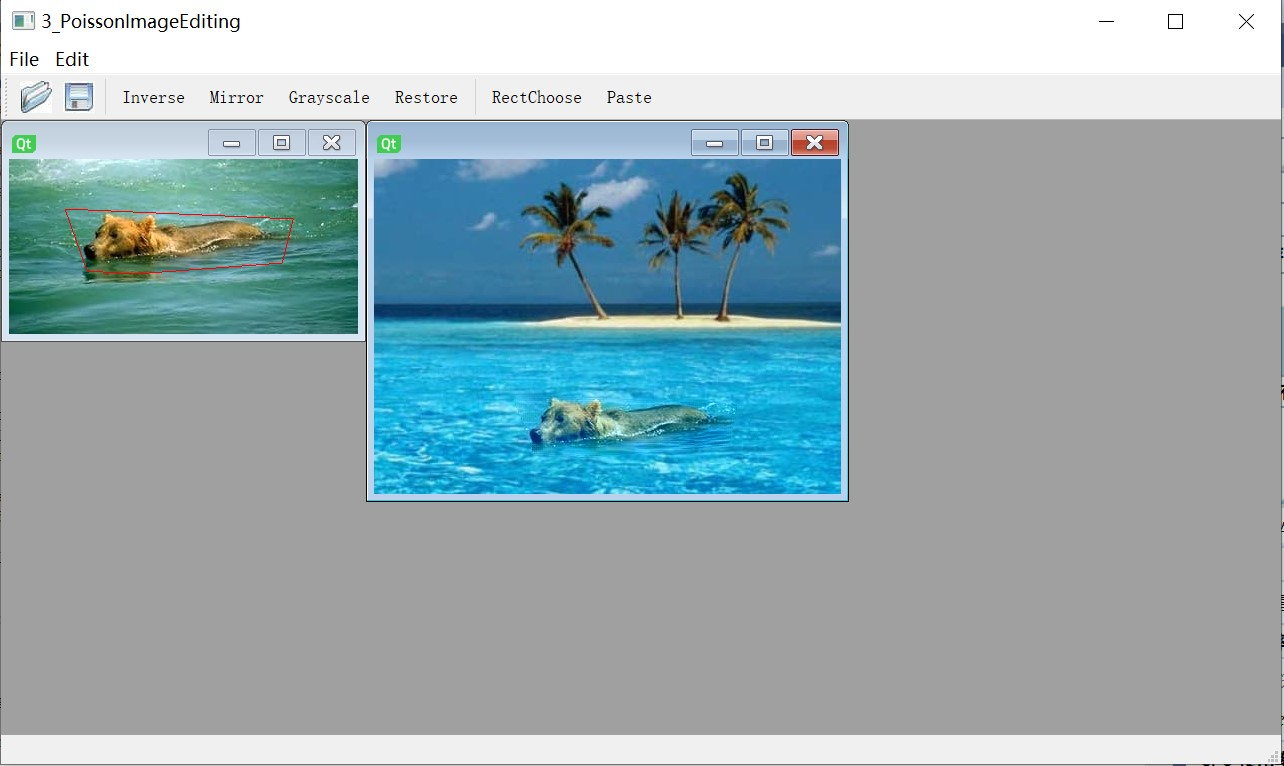
\includegraphics[width=4in]{possion.jpg}
		\end{center}
	\end{figure}
%	如上图。点击Select键后可以开始选择控制点(蓝色)和目标点(绿色),鼠标左键点击会画出控
%	制点,
%	再释放
%	就可以画出目标点(如下图)。之后可点击"IDW"键或"RBF"来进行图像变形。复选框用于选择
%	是否去噪。
%	\begin{figure}[htb]
%		\begin{center}
%			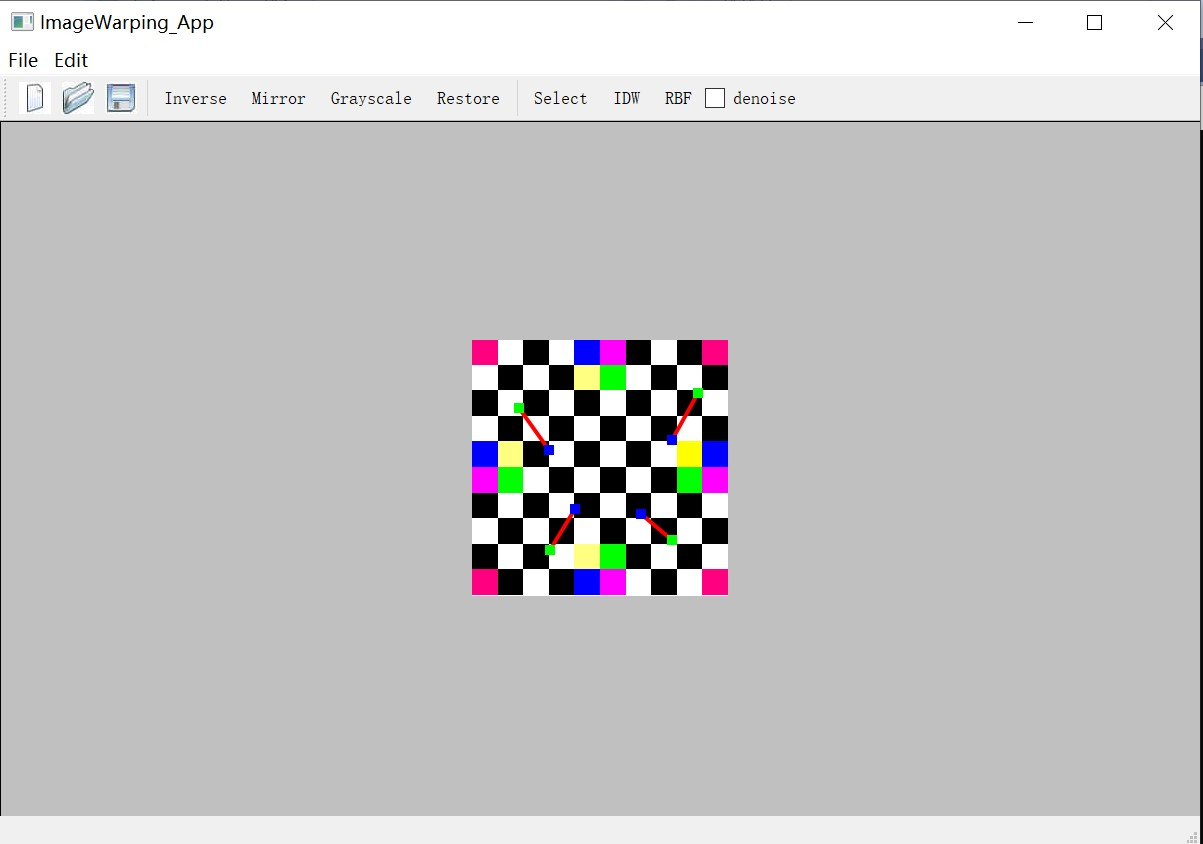
\includegraphics[width=4in]{ui1.jpg}
%		\end{center}
%	\end{figure}
%	\clearpage
%	\subsection{变形效果}
%	\begin{figure}[htbp]
%		\centering
%		\begin{minipage}{0.4\linewidth}
%			\centering
%			\caption{IDW}
%			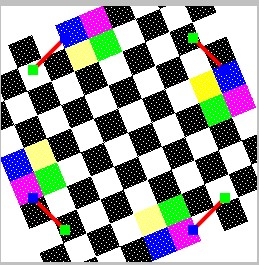
\includegraphics[width=1\linewidth]{IDW1.jpg}
%			\label{chutian1}
%		\end{minipage}
%		%\qquad
%		\begin{minipage}{0.4\linewidth}
%			\centering
%			\caption{RBF}
%			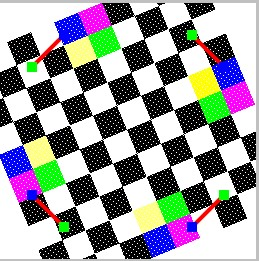
\includegraphics[width=1\linewidth]{RBF1.jpg}
%			\label{chutian2}
%		\end{minipage}
%	\end{figure}
%	\begin{figure}[htbp]
%		\centering
%		\begin{minipage}{0.4\linewidth}
%			\centering
%			\caption{IDW}
%			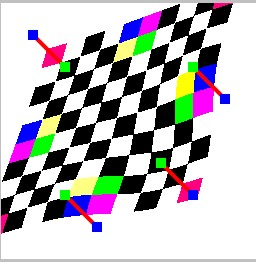
\includegraphics[width=1\linewidth]{IDW2.jpg}
%			\label{chutian1}
%		\end{minipage}
%		%\qquad
%		\begin{minipage}{0.4\linewidth}
%			\centering
%			\caption{RBF}
%			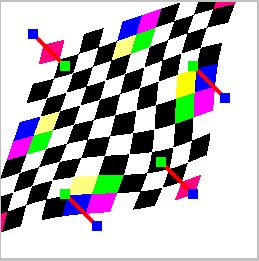
\includegraphics[width=1\linewidth]{RBF2.jpg}
%			\label{chutian2}
%		\end{minipage}
%	\end{figure}
%	\clearpage
%	\begin{figure}[htbp]
%		\centering
%		\begin{minipage}{0.4\linewidth}
%			\centering
%			\caption{IDW}
%			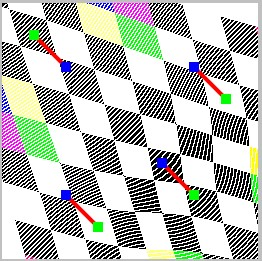
\includegraphics[width=1\linewidth]{IDW3.jpg}
%			\label{chutian1}
%		\end{minipage}
%		%\qquad
%		\begin{minipage}{0.4\linewidth}
%			\centering
%			\caption{RBF}
%			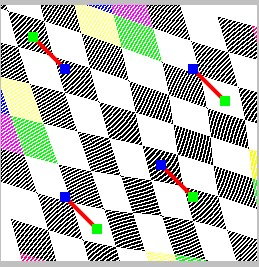
\includegraphics[width=1\linewidth]{RBF3.jpg}
%			\label{chutian2}
%		\end{minipage}
%	\end{figure}



	\section{不足}
	没有采用插值的方法来补缝。
\section{参考文献}
  $[1]$Ruprecht D, Muller H. [**Image warping with scattered data 
  interpolation**]IEEE Computer Graphics and Applications, 1995, 15(2): 37-43.
  
  $[2]$Arad N, Reisfeld D. [**Image warping using few anchor points and radial 
  functions**][C]//Computer graphics forum. Edinburgh, UK: Blackwell Science 
  Ltd, 1995, 14(1): 35-46.
\end{document}
